\section{Impletemention}
We have implemented and tested Viscous protocol using C++ language in linux\footnote{Our implementation may not work in other Unix based kernel. There is some dependency from Linux kernel.} kernel environment with pthread. We have performed most of the experiment in network emulator Mininet and real network using raspberry pis. 

Before we go deep into implementation, we will discuss the packet structure being used in our implementation.

\subsection{Packet Structure}
In Fig.~\ref{fig:packet_format}, we have depicted the packet structure we use in our implementation. \acrshort{tcp} packet structure influences our packet structure. Each packet is divided into three parts. They are a) mandatory header, b) variable length optional headers for additional information, and c) data region.

\begin{figure}[h!]
    \centering
    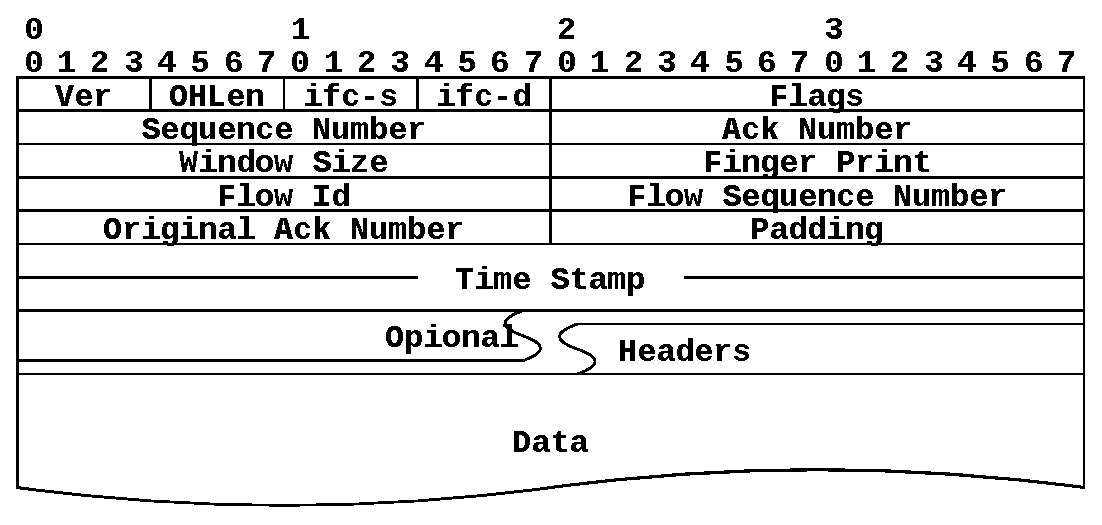
\includegraphics[width=1\linewidth]{img/Packet_format.eps}
    %\framebox[0.9\linewidth]{\input{img/Packet_format.tex}}
    \caption{Viscous packet header structure}
    \label{fig:packet_format}
\end{figure}
\subsubsection{Mandatory header}
Every packet starts with 28 bytes mandatory headers. It several fields. These fields are:
\begin{itemize}
    \item \textbf{Ver}: 4 bit protocol version number. The current version is 1.
    
    \item \textbf{OHLen}: 4 bit optional header count. We can accommodate at most 16 optional headers in a packet. As optional header size are different, it makes sense to store the number of optional headers than total size of it.
    
    \item \textbf{Ifc\_s}: 4 bit application defined source interface id.
    \item \textbf{Ifc\_d}: 4 bit application defined destination interface id.
    
    \hspace{3pt} Each application can use the device and list down the interface ids available. We assume that a device cannot have more than 15 interfaces. Interface ids start with 1. Interface id $0$ (zero) means it is not a valid interface. In our implementation, we use a pair of local and remote interface id as channel identifier. So, our implementation can support at most ($15\times15$) $225$ channels.
    
    \item \textbf{Flag}: Set of 1 bit flags. We will discuss it later in this section.
    
    \item \textbf{Sequenc Number}: 16-bit sequence number for a packet for a single packet. This sequence number is packet sequence number, not octet. We are using packet based sequence number because of two reasons: a) Packets are not created by channel handler and b) As we multiplex multiple flows, it is easier to track a packet from a flow than an octet from a flow.Sequence numbers are used by channel handler to provides reliable communication between two application. Two channel can have (and will have) same sequence number.
    
    \item \textbf{Ack Number}: 16 bit acknowledge number. It cumulative acknowledgment number like \acrshort{tcp} acknowledgment number. It denotes that, the receiver receives contiguous packet up to this sequence number and it did not receive next packet until the time it was sent from the receiver.
    
    \item \textbf{Window Size}: Reciever's advertise window.
    
    \item \textbf{Finger Print}: It is client's unique id generated by the server. Every packet includes this field except the $SYN$ packet. Packets will be discarded silently if this field is 0 (zero) or if there are no connection matching this fingerprint (i.e. invalid fingerprint).
    
    \item \textbf{Flow Id}: 16 bit flow id. To keep implementation simple, we use a 16bit integer as the flow identifier.
    
    \item \textbf{Flow Sequence Number}: 16-bit sequence number of each flow. It is independent of the sequence number. It requires at the flow layer to reorder packet at the receiver side. Similar reason as the sequence number, we use packet based flow sequence number.
    
    \item \textbf{Original Ack Number}: Viscous uses selective acknowledge mechanism. When the receiver receives an out of order packet, it is supposed to send duplicate acknowledgment packet acknowledging last conscious packet received. The receiver will put original sequence number of the packet which triggers the duplicate acknowledgment. This field gives sender an indication about packets received at the receiver side. So, send will no resend them again. It helps Viscous in reducing overall retransmission.
    
    \item \textbf{Padding}: It is not a field.
    
    \item \textbf{Sent timestamp}: When a sender sends a data packet it includes a current Unix timestamp in microseconds ($\mu s$). When a receiver receives a data packets, it includes this timestamp with ack packet. It helps sender in measuring round trip time ($rtt$) more accurately.
\end{itemize}

\subsubsection{Flags}
In our implementation, we reserve 16bit for several 1bit flags. Although we can use 16 different flags, currently we are using only eight flags. Figure \ref{fig:flags} gives an illustration of every flag and their position in bit fields. These flags are:
\begin{figure}[!h]
    \centering
    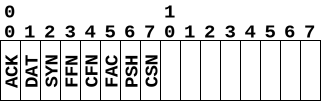
\includegraphics[width=.5\linewidth]{img/flags}
    \caption{Flags in Viscous packet header}
    \label{fig:flags}
\end{figure}

\begin{itemize}
    \item \textbf{$ACK$}: Acknowledgement flag. Describes that the packet contains acknowledgment number.
    \item \textbf{$DAT$}: Data flag. In our implementation, a packet will go up to flow layer only if packets marked as DATA packet.
    \item \textbf{$SYN$}: Synchronisation flag. Used for connection establishment.
    \item \textbf{$FFN$}: Flow finished indicator. We use it to close a single flow.
    \item \textbf{$CFN$}: Connection/client finish flag. We use it for connection closure.
    \item \textbf{$FAC$}: Flow acknowledgement. Not being used now.
    \item \textbf{$PSH$}: Push flag. It is the indicator that flow just started i.e. this is the first packet of a flag.
    \item \textbf{$CSN$}: Channel Synchronisation flag. It is being used when we try to set up a channel. It is the first packet; every channel sends to another end. It is two-way handshaking, not three-way.
\end{itemize}


\subsection{Modules and Layers}
We have developed several modules to perform different purposes throughout the lifetime of the protocol. Block diagram at figure \ref{fig:ProtocolDiagram} gives an elaborate description of our modular implementation.

\begin{figure}[!h]
    \centering
    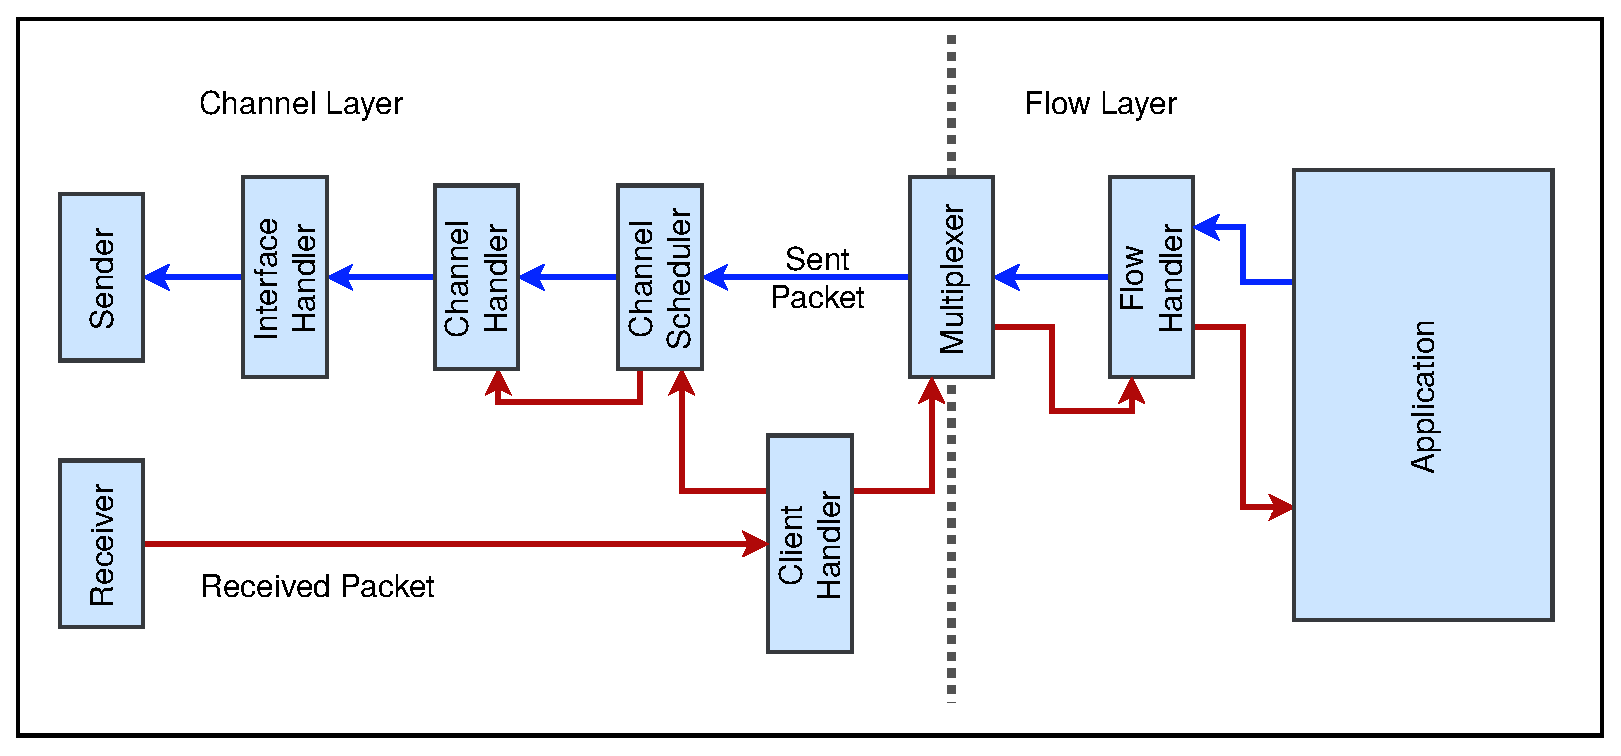
\includegraphics[width=.9\linewidth]{img/ModularDiagram}
    \caption{Internal Packet/Data flow diagram}
    \label{fig:ModularDiagram}
\end{figure}

Now we describe each module in detail.

\subsubsection{Application}
An application is the users' application using the Viscous library. Viscous exposes few \acrshort{api}s like a) start the client, b) add new flow, c)send data, d) stop/finish flow, d) stop client. These are the methods; the application needs to access Viscous library. Few \acrshort{api}s are provided via callbacks. These are a) new client added, b) new flow received, c) data received, d) flow closed. We use callback based \acrshort{api}s because it is easier to implement. It is expected that callback methods will be brief. Otherwise, it can degrade overall performance.


\subsubsection{Flow Handler}
Application directly sends data to this module and receives from it. Flow handler packetizes the raw data from the application and sends packets to lower layer for further processing. It does not need to store any outgoing packets as channel layer ensures the reliability. It only keeps track of the packets it sends to control the flow rate.

It reorders the out of packets it receives from the lower layer. There is a receives buffer that store out-of-order packets. This buffer is an array of packets. The first index point to the next expected packet sequence. Whenever flow-handler receives one or more contiguous packets from expected sequence, it delivers the data from those to the application.

There are one independent flow handler instances for each of the flows.

\subsubsection{Multiplxer}
The multiplexer is responsible for multiplexing the outgoing packets from multiple flows and forwards it to the packet scheduler. It is also responsible for demultiplexing incoming packet and forward them to appropriate flow handler. In the event of unknown flow id in the incoming packet, it simply creates a new flow handler for the new packet. Validation of the packet done mainly by channel handler.

\subsubsection{Client Handler}
Client handler is the manager of Viscous protocol \acrshort{api}. All incoming packets go through this module. For incoming packets, it checks packets validity using the fingerprint. 

After validation, it forwards each incoming packet to Channel Handler via channel scheduler for further validation and processing for congestion control algorithm. If channel handler return packet with marking as a valid packet, it forwards the packet to the multiplexer.

\subsubsection{Channel scheduler}
It schedules channel for the outgoing packet. It schedules outgoing packets to one of the channels. We used ack driven channel scheduler. A packet is scheduled to a channel only when the channel is capable of sending new packets i.e. after receiving the acknowledgment packet. \noteam{We need to give some reference. Sourav can help.}

\subsubsection{Channel Handler}
Channel handler is responsible for reliable communication and congestion controling in network. Instead of trying to build new congestion control algorithm, we tried follow standard \acrshort{tcp}\cite{RFC2582} congestion control algorithm. We mimic tcp new reno algorithm from RFC2582\cite{RFC2582} and other RFCs\cite{RFC2581,RFC2988,RFC2001,RFC0793} with some modifications. This modifications are as follows:
\begin{itemize}
    \item Channel handler handles packets, not byte-stream. So sequence number represents a packet, not a byte. We are using packet based sequence number because of following reasons: a) Packets are not created by channel handler and b) As we multiplex multiple flows, it is easier to track a packet from a flow than an octet from a flow.
    \item Each acknowledgment packet contains the original sequence number, that is the sequence number of the packet for which this acknowledgment triggered. It gives a similar effect as TCP Sack \cite{RFC2018}.
    \item We have modified the fast recovery phase describe in RFC2581\cite{RFC2582} with Sack modification. After receiving the first partial new acknowledgment, channel handler sends all the unacknowledged (via sack/original ack in the packet header) packet up to $recovery$ for each duplicate ack. This modification reduces retransmission due to timeout events when a run of packets get lost in the network.
\end{itemize}

\subsubsection{Receiver}
A receiver is an independent module run in an independent thread. Its only job is to wait for a datagram on a datagram socket (i.e. UDP socket). Whenever some packets arrive, it receives the packets and forwards to another module.

\subsubsection{Sender}
It is also an independent module. Only one instance can be there for an app. It looks at a common queue with channel handlers. Whenever some channel handler decides to send a packet, it put the packet in a common queue. Then sender picks up the packet from the queue and sends to the network.

We use packet-socket interface for sending purpose. There is no way define sending network interface in datagram socket \acrshort{api}. So, we encode Mac frame, then send it to the network. This method allows us to send through any interface we want.

Although using packet-socket we can send a packet through any interface we want, Unix network policy does not permit us. To overcome Unix systems problem, we follow the routing configuration\footnote{http://multipath-tcp.org/pmwiki.php/Users/ConfigureRouting} given by \acrshort{mptcp}.

%\subsection{Mobility}
%\noteam{write it down}